% Platform core -- the shared layer every hardware branch builds on.
%
% Build:  make -C slides platform_core.pdf
% Figures are produced by running the real pipeline:
%   python3 slides/figures/make_core_figures.py --out slides/figures

\documentclass[aspectratio=169,10pt]{beamer}
\usepackage{common/pdmtheme}
\graphicspath{{figures/}}

\title[Platform core]{Platform core}
\subtitle{Calibrated DSP, one feature contract, two implementations that agree}
\author{Predictive Maintenance Platform}
\date{13 October 2026}

\begin{document}

% ----------------------------------------------------------------- title ----
\begin{frame}[plain]
  \vspace{5mm}
  {\LARGE\bfseries Platform core}\\[2mm]
  {\large\color{pdmink2} Calibrated DSP, one feature contract, two
    implementations that agree}\par
  \vspace{5mm}\noindent{\color{pdmrule}\rule{\linewidth}{0.4pt}}\par
  \vspace{3mm}
  \begin{columns}[T]
    \begin{column}{0.45\textwidth}
      \scriptsize
      \kv{Python core}{64 tests, 28 modules}\\[1mm]
      \kv{C twin}{1\,049 golden-vector checks}\\[1mm]
      \kv{Code size}{9.6\,kB at \texttt{-Os}}\\[1mm]
      \kv{RAM}{85\,kB for a 4096-point pipeline}\\[1mm]
      \kv{Wire frame}{300\,B, CRC-32, versioned}\\[1mm]
      \kv{End-to-end POC}{\texttt{app.py -\/-replay}}
    \end{column}
    \begin{column}{0.47\textwidth}
      \scriptsize\color{pdmink2}
      Every number in this deck is produced by running the code at build time.
      \\[2mm]
      Every number is also \textbf{from simulated data}. No model here has been
      validated on measured data; no firmware here has run on hardware. Both
      gaps are stated where they matter and listed in
      \texttt{docs/07\_production\_readiness.md}.
    \end{column}
  \end{columns}
  \srcnote{Branch \texttt{platform/core}.}
\end{frame}

% ------------------------------------------------------- the one decision ---
\begin{frame}{The decision everything else follows from}
  \begin{columns}[T]
    \begin{column}{0.49\textwidth}
      \centering
      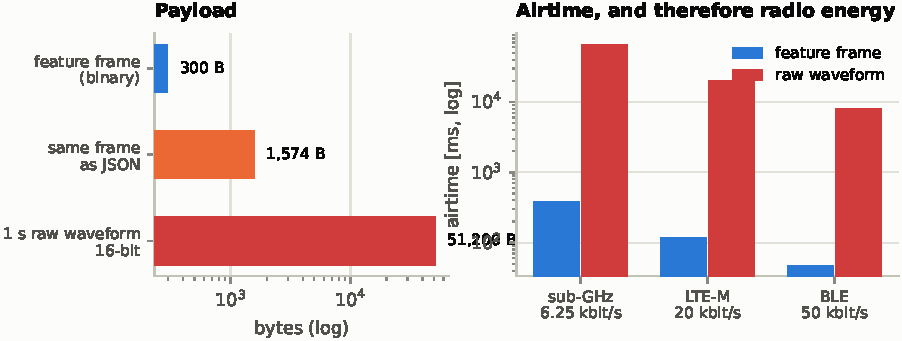
\includegraphics[width=\linewidth]{core_payload.pdf}
    \end{column}
    \begin{column}{0.47\textwidth}
      \small
      \textbf{Features on the radio, waveforms only on demand.}
      \\[2mm]
      \scriptsize
      A 1\,s, 25.6\,kHz, 16-bit acquisition is 51\,kB. The feature frame is
      300\,B --- \textbf{170$\times$ smaller}. Radio energy dominates a battery
      sensor's budget, so that ratio is the battery life.
      \\[2mm]
      Consequences, all of them forced:
      \\[1mm]
      $\bullet$ The frame must support \emph{diagnosis}, not just detection ---
      hence 63 features including bearing-frequency evidence, not 6 summary
      statistics. The information is destroyed at the device; the cloud cannot
      reconstruct it.\\[1mm]
      $\bullet$ The edge needs a real FFT, envelope demodulation and a model.
      Hence \texttt{cdsp/}.\\[1mm]
      $\bullet$ Edge and cloud must compute \emph{identical} features, or trends
      break at the boundary between a live frame and a recomputed snapshot.
    \end{column}
  \end{columns}
  \takeaway{A 170$\times$ payload ratio is not an optimisation, it is the
    architecture. Everything hard about this project follows from it.}
\end{frame}

% -------------------------------------------------------------- calibration -
\begin{frame}{Calibration is not a detail, and it is testable}
  \begin{columns}[T]
    \begin{column}{0.56\textwidth}
      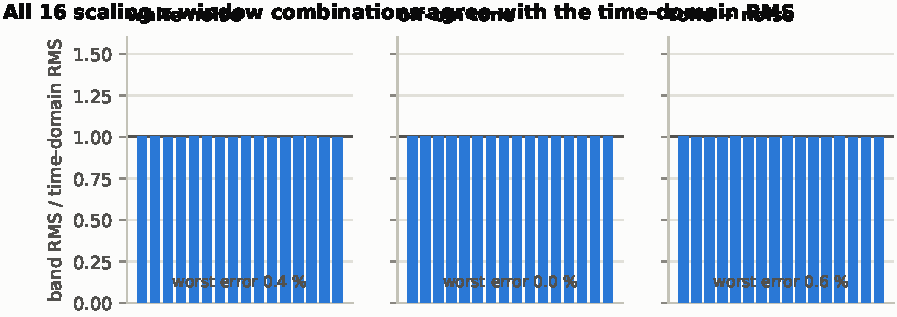
\includegraphics[width=\linewidth]{core_calibration.pdf}
      \\[1mm]
      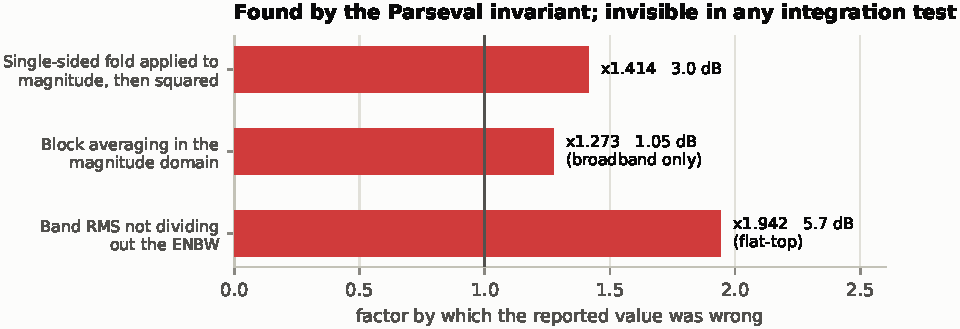
\includegraphics[width=\linewidth]{core_calibration_bugs.pdf}
    \end{column}
    \begin{column}{0.41\textwidth}
      \small The invariant
      \\[1mm]
      \scriptsize
      Band RMS over the full band must equal the time-domain RMS --- for
      \emph{every} scaling (\texttt{peak}, \texttt{rms}, \texttt{power},
      \texttt{psd}) and \emph{every} window. 16 combinations, three signal types.
      \\[2mm]
      It must also read a single tone's amplitude correctly. One function, both
      properties: that is what forces the maths to be right rather than merely
      self-consistent.
      \\[3mm]
      \small Three bugs it caught
      \\[1mm]
      \scriptsize
      Each was invisible in an integration test, consistent across the whole
      codebase (so every internal comparison agreed), and would have been wrong
      by a constant factor \textbf{forever} --- discovered the first time
      somebody compared the dashboard to a calibrated handheld meter.
      \\[2mm]
      The $\pi/4$ one is the nastiest: averaging magnitudes instead of power
      biases \emph{broadband content only}. Tones were correct. Only the noise
      floor was 1\,dB low.
    \end{column}
  \end{columns}
\end{frame}

% ---------------------------------------------------------- two implementations
\begin{frame}{Two implementations, held together by generated vectors}
  \centering
  \begin{tikzpicture}[node distance=5mm and 10mm]
    \node[pdmblk, minimum width=30mm] (py) {\texttt{core/pdmcore.dsp}\\\tiny float64, reference};
    \node[pdmblk3, minimum width=26mm, right=28mm of py] (c) {\texttt{cdsp/}\\\tiny float32, C99, no malloc};
    \node[pdmblkoff, minimum width=24mm, below=13mm of $(py)!0.5!(c)$] (g) {\texttt{tests/golden.h}\\\tiny 1\,049 checks};
    \draw[pdmarrow] (py.south) |- (g.west);
    \node[pdmnote, below left=1mm and -4mm of py.south] {\tiny gen\_golden.py};
    \draw[pdmarrow] (g.east) -| (c.south);
    \node[pdmnote, below right=1mm and -4mm of c.south] {\tiny test\_cdsp.c};
    \node[pdmnote, right=4mm of c, align=left] {\tiny runs on the build host,\\\tiny every commit,\\\tiny no hardware};
  \end{tikzpicture}
  \\[3mm]
  \begin{columns}[T]
    \begin{column}{0.48\textwidth}
      \scriptsize
      \textbf{Why bother.} A maintenance decision must not depend on
      \emph{where} the number was computed. If the MCU and the cloud disagree,
      every threshold, baseline and trend is quietly wrong in a way that is
      almost impossible to debug from a dashboard.
      \\[2mm]
      Tolerances are per-check and justified: the expected float32 accumulation
      error for that specific operation, not ``close enough''. A tolerance that
      has to be loosened is a signal.
    \end{column}
    \begin{column}{0.48\textwidth}
      \scriptsize
      \textbf{It caught a bug nothing else would have.} The FFT twiddle table
      was allocated \texttt{3n/4} floats where the algorithm needs
      \texttt{n+2}. The split-stage table overflowed into itself and corrupted
      \textbf{exactly bins $n/8+1 \ldots 3n/8$} of every transform.
      \\[1.5mm]
      Bins outside that range were perfect. A tone sweep would have passed.
      Parseval over the full band would have passed. A spectrum plot would have
      looked plausible.
      \\[1.5mm]
      395 of 1\,049 checks failed and pointed straight at it.
    \end{column}
  \end{columns}
  \takeaway{Hence \texttt{PDM\_RFFT\_TWIDDLE\_LEN(n)} --- size the table with the
    macro, never by hand.}
\end{frame}

% ------------------------------------------------------------------ budget ---
\begin{frame}{What the device actually pays}
  \begin{columns}[T]
    \begin{column}{0.56\textwidth}
      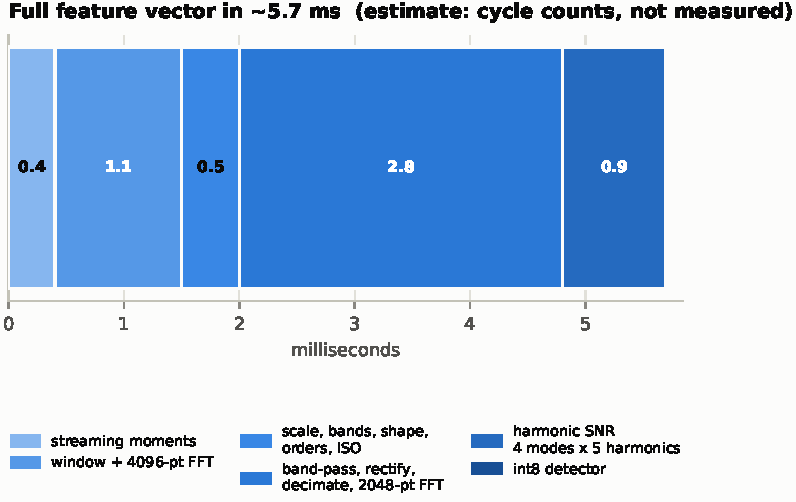
\includegraphics[width=\linewidth]{core_budget.pdf}
    \end{column}
    \begin{column}{0.41\textwidth}
      \scriptsize
      \begin{tabular}{@{}lr@{}}
        \toprule
        \textbf{Code} (\texttt{-Os}) & \\
        \midrule
        \texttt{pdm\_envelope.o} & 2\,132 B \\
        \texttt{pdm\_spectrum.o} & 1\,996 B \\
        \texttt{pdm\_features.o} & 1\,556 B \\
        \texttt{pdm\_fft.o} & 1\,348 B \\
        \texttt{pdm\_bearing.o} & 1\,108 B \\
        \texttt{pdm\_model.o} & 868 B \\
        \texttt{pdm\_window.o} & 636 B \\
        \midrule
        \textbf{total} & \textbf{9\,644 B} \\
        \bottomrule
      \end{tabular}
      \\[2mm]
      \textbf{RAM} for a 4096-point pipeline: \textbf{85\,kB} (window, twiddle,
      bit-reversal, in-place FFT buffer, magnitude, spectrum, envelope, model
      scratch).
      \\[2mm]
      Fits STM32U585, nRF9160, ESP32-S3, RA8D1, Alif E7. Does \emph{not} fit a
      64\,kB part; the documented fallback is \texttt{n\_fft} 2048 --- 43\,kB,
      6.25\,Hz resolution instead of 3.125\,Hz.
      \\[2mm]
      At one acquisition per hour, 5.7\,ms is a \textbf{1.6\,ppm} compute duty
      cycle. The radio and the sensor's settling time dominate, not the DSP ---
      which is what justifies doing full envelope analysis on the device.
    \end{column}
  \end{columns}
  \srcnote{Code size and RAM are measured. The millisecond figures are estimates
    from cycle counts and CMSIS-DSP benchmarks --- no board has been flashed.}
\end{frame}

% --------------------------------------------------------------- detectors ---
\begin{frame}{Detectors, and the three things the table really says}
  \centering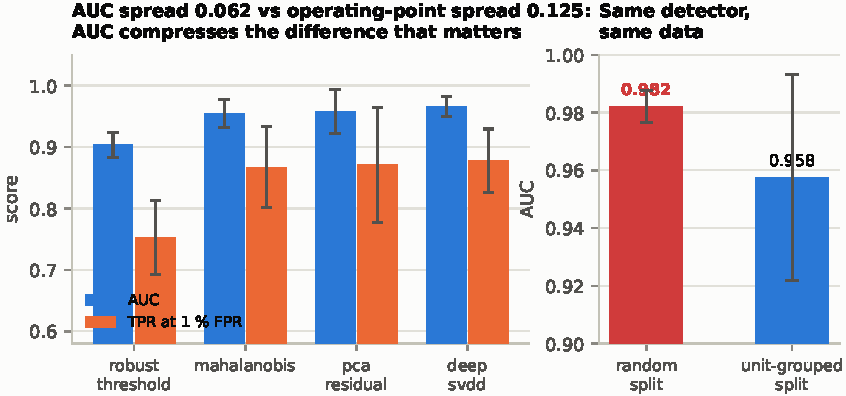
\includegraphics[width=0.80\linewidth]{core_detectors.pdf}
  \\[1mm]
  \begin{columns}[T]
    \begin{column}{0.32\textwidth}
      \scriptsize
      \textbf{1. The top three are not separable.} Within one standard
      deviation on every metric. Choose on explainability and footprint, not on
      these numbers.
    \end{column}
    \begin{column}{0.32\textwidth}
      \scriptsize
      \textbf{2. AUC hides what matters.} AUC spread 0.062; spread at 1\,\% FPR
      \textbf{0.125}. \texttt{robust\_threshold} gives up 6 points of AUC and
      \textbf{12 of recall}.
    \end{column}
    \begin{column}{0.32\textwidth}
      \scriptsize
      \textbf{3. The split beats the model.} And a leaky split looks
      \emph{more} reproducible ($\pm$0.005 vs $\pm$0.036) --- which is how it
      survives review.
    \end{column}
  \end{columns}
  \srcnote{Simulated fleet: 3 machine classes $\times$ 3 units, 594
    acquisitions, 7 split seeds, \texttt{leakage\_report} clean on every one.
    $\pm3$\,\% speed jitter per unit so no model can memorise a shaft frequency.}
\end{frame}

% ------------------------------------------------------------- degradation ---
\begin{frame}{90 days to failure}
  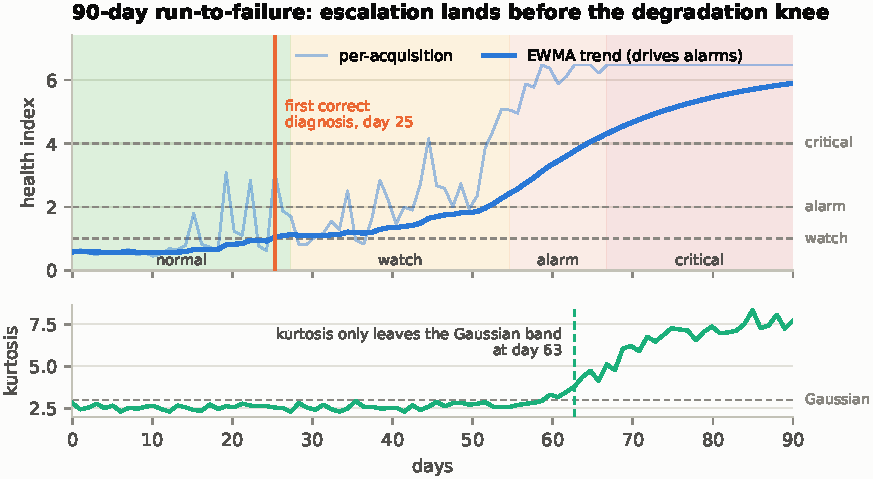
\includegraphics[width=0.95\linewidth]{core_degradation.pdf}
  \\[1mm]
  \begin{columns}[T]
    \begin{column}{0.48\textwidth}
      \scriptsize
      \begin{tabular}{@{}lr@{}}
        \toprule
        First correct diagnosis & day 25 \\
        \texttt{normal} $\rightarrow$ \texttt{watch} & day 27 \\
        $\rightarrow$ \texttt{alarm} & day 55 \\
        $\rightarrow$ \texttt{critical} & day 67 \\
        \midrule
        Kurtosis leaves the Gaussian band & day 63 \\
        \bottomrule
      \end{tabular}
    \end{column}
    \begin{column}{0.48\textwidth}
      \scriptsize
      \textbf{The last row is the point.} Kurtosis is the textbook early
      bearing indicator. Here the fused index escalates \textbf{36 days before
      kurtosis moves at all}, because the index also sees the high-frequency
      band energy, which rises first.
      \\[1.5mm]
      A programme that watches kurtosis alone loses five weeks --- and then, as
      the defect spreads over the raceway, kurtosis falls back toward 3 and the
      machine looks like it is recovering.
    \end{column}
  \end{columns}
  \takeaway{Hysteresis, $n$-of-$m$ confirmation and a minimum dwell are what turn
    the noisy per-acquisition index into three state changes instead of forty.}
\end{frame}

% ------------------------------------------------------------- health chain --
\begin{frame}{The chain, and where it is allowed to abstain}
  \centering
  \begin{tikzpicture}[node distance=4mm and 5mm]
    \node[pdmblk, minimum width=19mm] (f) {63 features};
    \node[pdmblk, minimum width=19mm, right=of f] (b) {operating\\baseline};
    \node[pdmblk2, minimum width=19mm, right=of b] (h) {health\\index};
    \node[pdmblk2, minimum width=19mm, right=of h] (a) {alarm state\\machine};
    \node[pdmblk3, minimum width=19mm, right=of a] (d) {rule\\diagnosis};
    \node[pdmblk3, minimum width=19mm, right=of d] (r) {RUL};
    \node[pdmblk, minimum width=19mm, right=of r] (w) {work\\order};
    \foreach \x/\y in {f/b, b/h, h/a, a/d, d/r, r/w} \draw[pdmarrow] (\x) -- (\y);
    \node[pdmnote, below=2mm of b, align=center] {\tiny ``unknown''\\\tiny until 40 frames};
    \node[pdmnote, below=2mm of d, align=center] {\tiny \texttt{unclassified}\\\tiny is an answer};
    \node[pdmnote, below=2mm of r, align=center] {\tiny \texttt{insufficient}\\\tiny \texttt{\_evidence}};
  \end{tikzpicture}
  \\[3mm]
  \begin{columns}[T]
    \begin{column}{0.32\textwidth}
      \scriptsize
      \textbf{Abstention is a feature.}\\
      An asset inside its commissioning window is \emph{unknown}, not healthy,
      and no alarm can fire. The RUL filter returns
      \texttt{insufficient\_evidence} far more often than a number. Diagnosis
      can return \texttt{elevated\_vibration\_unclassified}.
      \\[1mm]
      ``The level is high and we do not yet know why'' is a legitimate and
      useful output. A confidently wrong fault label is not.
    \end{column}
    \begin{column}{0.32\textwidth}
      \scriptsize
      \textbf{The baseline adapts only while NORMAL.}\\
      Mounts relax, grease redistributes, ambient temperature moves 25\,K with
      the seasons --- a frozen baseline becomes a false-alarm generator.
      \\[1mm]
      But adaptation gated on \emph{time} absorbs a developing fault into
      ``normal'' and hides exactly what it was built to find. Gating on
      \emph{state} is what makes it safe.
    \end{column}
    \begin{column}{0.32\textwidth}
      \scriptsize
      \textbf{Feed RUL an amplitude, not the index.}\\
      The health index is capped so the alarm logic saturates sensibly. An
      exponential fit to a saturating signal concludes the crossing already
      happened.
      \\[1mm]
      So prognostics consume \texttt{band.10\_rms} normalised to its healthy
      median, and ``failure'' is defined as 20$\times$ the healthy
      high-frequency level --- a statement about the asset, not about the index.
    \end{column}
  \end{columns}
\end{frame}

% ------------------------------------------------------------------ e2e ------
\begin{frame}[fragile]{End to end, with no infrastructure}
\begin{lstlisting}[language=bash]
$ python3 cloud/ingest/app.py --replay
      day   sev    HI  trend     state  diagnosis                      RUL
     28.3  0.01  0.78   1.06     watch  -                              insufficient_evidence
     42.5  0.02  1.72   1.31     watch  bearing_outer_race (0.80)      insufficient_evidence
     56.6  0.05  5.38   2.53     alarm  bearing_outer_race (1.00)      insufficient_evidence
     70.8  0.19  6.47   4.61  critical  bearing_outer_race (1.00)      already_failed

validation checks
  corrupted CRC      -> rejected
  CLIPPED flag       -> rejected
  replayed sequence  -> deduplicated
  silent for 115 d   -> stale alarm raised
\end{lstlisting}
  \scriptsize
  The device side encodes real 300-byte wire frames; the ingest side runs the
  same \texttt{handle\_raw()} the MQTT and HTTP transports call. No broker, no
  database, no Docker.
  \\[2mm]
  \textbf{The four lines at the bottom are the ones that matter.} A POC that
  only demonstrates the happy path has not demonstrated the thing that matters:
  a clipped acquisition scored as an anomaly, or a store-and-forward replay
  re-driving the alarm machine, are the failures that destroy trust in a
  deployment --- and they are invisible until they happen in the field.
\end{frame}

% ------------------------------------------------------------------ gaps -----
\begin{frame}{What is not true yet}
  \small
  \begin{columns}[T]
    \begin{column}{0.48\textwidth}
      \textbf{Easy to believe, and false}
      \\[1.5mm]
      \scriptsize
      $\bullet$ \textbf{``The firmware works.''} Structurally complete, DSP
      verified against a reference. \emph{Never flashed to a board.}\\[1mm]
      $\bullet$ \textbf{``The models are good.''} 0.90--0.97 AUC on
      \emph{simulated} data. The simulator was written by the same process that
      wrote the features, so some agreement is self-fulfilling.\\[1mm]
      $\bullet$ \textbf{``The timings are measured.''} Code size and RAM are.
      The millisecond figures are cycle-count estimates.\\[1mm]
      $\bullet$ \textbf{``The power budgets are measured.''} Datasheet
      arithmetic. Reality is typically 20--50\,\% worse.\\[1mm]
      $\bullet$ \textbf{``The compose stack runs.''} Never started --- no Docker
      in this environment.
    \end{column}
    \begin{column}{0.48\textwidth}
      \textbf{Next five, in order}
      \\[1.5mm]
      \scriptsize
      \textbf{1. Cross-compile in CI.} $\sim$20 lines per kit. Until the firmware
      compiles for its target, ``complete'' is a claim about structure. Nothing
      else on this list matters more.\\[1mm]
      \textbf{2. Validate on CWRU and MFPT} with bearing-wise partitioning. Data
      is public, harness exists. Until then every detection number here is about
      a simulator.\\[1mm]
      \textbf{3. Write the int8 export tool.} The inference path is pinned by
      golden vectors; nothing converts a trained detector into the C arrays.
      That is the missing link between training and the device.\\[1mm]
      \textbf{4. Wire ingest to Postgres.} Schema complete, service holds work
      orders in memory. No transactional write means no audit trail.\\[1mm]
      \textbf{5. Adopt arXiv 2607.08273's} regime-based split and residual
      calibration. Closest published work to this problem, MIT-licensed.
    \end{column}
  \end{columns}
  \srcnote{Full assessment with a per-item state:
    \texttt{docs/07\_production\_readiness.md}.}
\end{frame}

\end{document}
